\chapter{Domain Analysis}
\label{cha:analysis}

This chapter analyzes the concepts of services and service decomposition in more detail and concludes with a questionnaire that helps to assess decompositions. 

\section{Service Definition}
\label{sec:serviceIntro}

\textit{Service} is one of the most used terms in the field of software architecture and has been defined differently in many papers, books, and blog posts in numerous ways and various contexts. This section consolidates multiple definitions and defines service for this thesis.

\subsection{Different Views on Services}

The \enquote{4+1 View Model of Software Architecture} by Philippe Kruchten\cite{fourPlusOne} describes software architecture using the views \textit{Logical View}, \textit{Physical View}, \textit{Development View}, and \textit{Process View} which are illustrated by \textit{Scenarios}. During our research we discovered that the difficulty to clearly define the word service lies in the fact that different definitions focus on contrasting views. For this thesis we use multiple definitions for the term service depending if we write about the \textit{logical} or the \textit{physical} view of a service.

\subsubsection{Logical Service}

\begin{quotation}
\textit{A service is the technical authority for a specific business capability} \newline --- Udi Dahan\cite{serviceDefinitionDahan}
\end{quotation}
   
This definition focuses more on the logical or scenario view of a service than its technical representation. He further defines that all data and operations required to provide a business capability are owned by one and only one service. 

Udi Dahan implies that a service is not restricted to a specific application, process, technology or layer. In fact, it contains required layers itself, including databases, logic, and \gls{UI} code.

A logical service is autonomous and composed from many processes, webservices or databases, but keeps a clear boundary and interface against the outer world. Communication with other parts of the system only happens on a well defined interface on a common communication channel.

\subsubsection{Bounded Context}

Another concept describing logical services is the bounded context as defined in the Domain-Driven Design\cite{evans2014domain}:

\begin{quotation}
	\textit{A description of a boundary (typically a subsystem, or the work of a particular team) within which a particular model is defined and applicable.}
\end{quotation}

A model only used within one bounded context is defined and visible only in that context. Accordingly, a model used in multiple services needs to have a globally shared definition, defined as \textit{Published Language} in the context of \gls{DDD}\cite{evans2014domain}:

\begin{quotation}
	\textit{The translation between the models of two bounded contexts requires a common Language.}
\end{quotation}

The process of service decomposition as done by the Service Cutter automatically defines the published language of the system. 

\subsubsection{Physical Service}

Martin Fowler describes a service as following:

\begin{quotation}
	\textit{A service will be used remotely through some remote interface, either synchronous or asynchronous.}\cite{fowlerIoC}
\end{quotation}

This definition by Martin Fowler is based on the physical structure and is close to what recently has been advertised as a \textit{microservice}:

\begin{quotation}
	\textit{In short, the microservice architectural style is an approach to developing a single application as a suite of small services, each running in its own process and communicating with lightweight mechanisms, often an HTTP resource API.}\cite{fowlerMicroservice}
\end{quotation}

A process providing a remote API might provide business logic, pure technical functionality or a data store. A service commonly includes at least a data store, wrapped by a RESTful HTTP API. Physical services might be congruent with logical services but very often more complex cases split logical services in multiple physical services. 

\subsubsection{Should the Service Cutter Produce Logical or Physical Service Candidates?}

The Service Cutter incorporates logical and physical aspects in the decomposition process but focuses more on the former. 

Not all reasons to create physical services can be analyzed in a structured way. The Service Cutter cannot decide if a service using a database runs in a single process or connects to its database over a remote interface. Similarly, an operations team might decide to run different logical services on the same machine or even in the same process to save resources and simplify deployment. These decisions are often reasoned by operational aspects rather than the system's characteristics. 

Nevertheless, some physical aspects can be analyzed. As an example, the Service Cutter is able to receive information about the storage requirements for the system's data. It suggests that data with very high storage requires an own service because a different database technology is necessary. 

We define that the Service Cutter focuses on logical services while incorporating physical aspects whenever possible. 

\subsection{Nanoentities, Building Blocks for Services}

Sam Newman writes in his book \textit{Building Microservices}\cite[p. 34]{newman2015building}: 

\begin{quote}
	\textit{When you start to think about the bounded contexts that exist in your organization, you should be thinking not in terms of data that is shared, but about the capabilities those contexts provide the rest of the domain.}
\end{quote}

In order to provide capabilities, a service needs resources. We identified three types of resources which are the building blocks of services:

\begin{description}
	\item[Data] A service has ownership over some of the system's data. It is the only instance responsible for changes on that data and optionally informs other services about changes. The data is often, but not necessarily, stored in a database. Data which is published to other services belongs to the published language of the system.
	\item[Operations] A service has ownership over business rules and calculation logic. These operations are often, but not necessarily, based on the data the service owns.
	\item[Artifacts] A service has ownership over artifacts. An artifact is a collection of data or operation results transformed into a specific format. An example is a business report which has been built using operations and data.
\end{description}

In order to enable a structured approach to service decomposition, we generalize these resources with the concept of a \textit{nanoentity}. Examples for possible nanoentities are illustrated in Figure \ref{fig:nanoentities}.

\begin{figure}[H]
	\centering{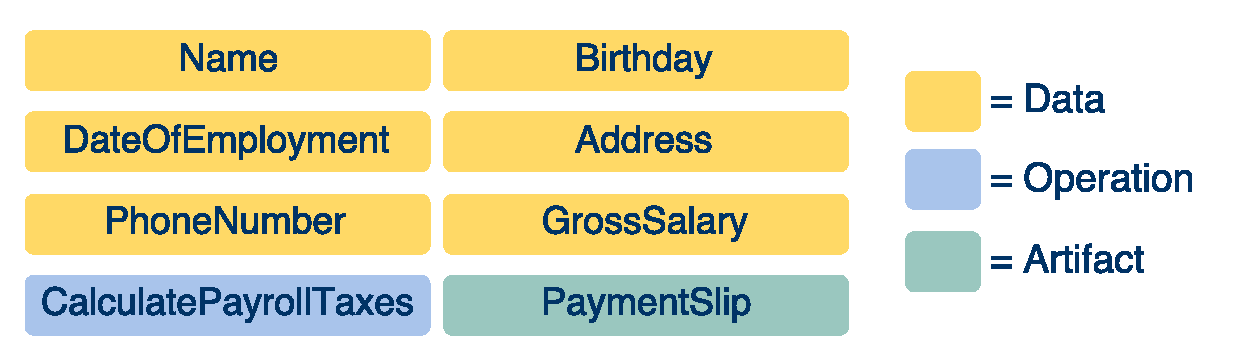
\includegraphics[scale=0.7]{diagrams/Nanoentities.pdf}}
	\caption{Nanoentities related to an employee.}
	\label{fig:nanoentities}
\end{figure}	

A service must contain  at least two type of nanoentities to be considered a logical service. 
\begin{itemize}
\item Something only providing CRUD\footnote{Create, Read, Update, and Delete} functions on data is considered a database. 
\item Something only providing operations is considered a function. 
\item Something only providing artifacts is considered a resource or a database. 
\end{itemize}

Service decomposition is the act of defining a number of services and assigning all nanoentities to the responsible service. The driving forces for decomposition are discussed in more detail in the next section.


\section{Service Decomposition}

Well experienced software architects decompose systems by reason of driving forces to ensure a maintainable, robust and consistent system with business relevance and good performance. This section describes the forces mostly considered by architects. 

Decomposition has been a main discipline for programmers since early in the history of our industry. David L. Parnas published a paper entitled \enquote{On the Criteria To Be Used in Decomposing Systems into Modules} in 1972\cite{parnaDecomposing}. Shortly after, the terms \textit{coupling} and \textit{cohesion} as software design metrics appeared as part of the \textit{Structured Design} technique\cite{structuredDesign}:

\begin{description}
	\item[Coupling] \textit{A measure of how closely connected two routines or modules are.\newline In	software design, a measure of the interdependence among modules in a computer program.}\cite{softwareVocabulary}
	\item[Cohesion] \textit{The manner and degree to which the tasks performed by a single software module are related to one another.} \newline 
	\textit{In software design, a measure of the strength of association of the elements within a module.}\cite{softwareVocabulary}
\end{description}

Software architects commonly started to use these metrics to define that good architectures have high cohesion within and low coupling between its parts. Robert Martin later described a general principle to achieve loose coupling and high cohesion:

\begin{description}
	\item[Single Responsibility Principle] \textit{Gather together the things that change for the same reasons. Separate those things that change for different reasons.}\cite{SRP}
\end{description}

Starting from these principles, we analyzed different types of coupling and cohesion and created the decomposition model described in the next chapter.

